\documentclass[10pt,a4paper]{article}
\usepackage[right=0.5cm, left=0.5cm,top=0.5cm,bottom=1.5cm]{geometry}
\usepackage{enumitem}
\usepackage{graphicx}
\usepackage{array, tasks}
\usepackage{blindtext}
\usepackage{amsmath,amsfonts,amssymb,mathrsfs,amsthm}
\usepackage{fancyhdr}
\usepackage{xcolor}
% \usepackage{booktabs}
% \usepackage[font={bf}]{caption}
% \captionsetup[table]{box=colorbox,boxcolor=orange!20}
% \usepackage{float}
% \usepackage{esvect}
% \usepackage{tabularx}
\usepackage{pifont}
\usepackage{colortbl}
\usepackage{fancybox}
\mathversion{bold}
\usepackage{pgfplots}
\usepackage{tikz}
 \usepackage[tikz]{bclogo}
 \usetikzlibrary{arrows.meta}
 \usepackage{mathpazo}
\usepackage{ulem}
\usepackage{yagusylo}
\usepackage{textcomp}
\usepackage{multicol}
\usepackage{varwidth}
\usetikzlibrary{calc,intersections}
\usepackage{pgfplots}
\pgfplotsset{compat=1.11}
\usepackage{tkz-tab}
\usepackage{xcolor}
\usepackage{color}
\usetikzlibrary{calc}
\usepackage{tikz}
% \mathcharDéfinition\times="2202
\usepackage[most]{tcolorbox} 
\definecolor{head}{RGB}{255,211,204}
\definecolor{problemblue}{RGB}{100,134,158}
\definecolor{exercisebgblue}{RGB}{192,232,252}
\definecolor{darkbrown}{rgb}{0.4, 0.26, 0.13}

\newcommand{\Lim}{\displaystyle\lim}
\makeatother
\newcommand{\oij}{$\left( \text{O};\vv{i},\vv{j} , \vv{k}\right)$}
\colorlet{darkred}{red!30!black}
\newcommand{\red}[1]{\textcolor{darkred}{ #1}}
\newcommand{\rr}{\mathbb{R}}
\renewcommand{\baselinestretch}{1.2}
 \setlength{\arrayrulewidth}{1.25pt}
\usepackage{titlesec}
\usepackage{titletoc}
\usepackage{minitoc}
\usepackage{ulem}
%--------------------------------------------------------------

\usetikzlibrary{decorations.pathmorphing}
\tcbuselibrary{skins}

%%%%%%%%%%%
%-------------------------------------------------------------------------
\tcbset{
        enhanced,
        colback=white,
        boxrule=0.1pt,
        colframe=brown!10,
        fonttitle=\bfseries
       }


\newcommand*{\arraycolor}[1]{\protect\leavevmode\color{#1}}
\newcolumntype{A}{>{\columncolor{blue!50!white}}c}
\newcolumntype{B}{>{\columncolor{LightGoldenrod}}c}
\newcolumntype{C}{>{\columncolor{FireBrick!50}}c}
\newcolumntype{D}{>{\columncolor{Gray!42}}c}

\newcounter{mysection}
\newcounter{mysubsection}
\newcommand{\mysection}[1]{%
    \stepcounter{mysection} % Increment the counter
    \textcolor{red}{\LARGE\themysection. #1 :}
}
\newcommand{\mysubsection}[2]{
    \stepcounter{mysubsection}
    \textcolor{red}{\large \themysection.#1. #2 :}
}
% \textcolor{red}{\LARGE\bfseries 1. Les équation du deuxiéme degrée :}

%------------------------------------------------------
\newtcolorbox[auto counter]{Définition}[1]{enhanced,
before skip=2mm,after skip=2mm,
colback=yellow!20!white,colframe=lime,boxrule=0.2mm,
attach boxed title to top left =
    {xshift=0.6cm,yshift*=1mm-\tcboxedtitleheight},
    varwidth boxed title*=-3cm,
    boxed title style={frame code={
                        \path[fill=lime]
                            ([yshift=-1mm,xshift=-1mm]frame.north west)  
                            arc[start angle=0,end angle=180,radius=1mm]
                            ([yshift=-1mm,xshift=1mm]frame.north east)
                            arc[start angle=180,end angle=0,radius=1mm];
                        \path[left color=lime,right color = lime,
                            middle color = lime]
                            ([xshift=-2mm]frame.north west) -- ([xshift=2mm]frame.north east)
                            [rounded corners=1mm]-- ([xshift=1mm,yshift=-1mm]frame.north east) 
                            -- (frame.south east) -- (frame.south west)
                            -- ([xshift=-1mm,yshift=-1mm]frame.north west)
                            [sharp corners]-- cycle;
                            },interior engine=empty,
                    },
fonttitle=\bfseries\sffamily,
title={#1 ~\thetcbcounter}}
%------------------------------------------------------
\newtcolorbox[auto counter]{Proposition}{enhanced,
before skip=2mm,after skip=2mm,
colback=yellow!20!white,colframe=blue,boxrule=0.2mm,
attach boxed title to top left =
    {xshift=0.6cm,yshift*=1mm-\tcboxedtitleheight},
    varwidth boxed title*=-3cm,
    boxed title style={frame code={
                        \path[fill=blue]
                            ([yshift=-1mm,xshift=-1mm]frame.north west)  
                            arc[start angle=0,end angle=180,radius=1mm]
                            ([yshift=-1mm,xshift=1mm]frame.north east)
                            arc[start angle=180,end angle=0,radius=1mm];
                        \path[left color=blue,right color = blue,
                            middle color = blue]
                            ([xshift=-2mm]frame.north west) -- ([xshift=2mm]frame.north east)
                            [rounded corners=1mm]-- ([xshift=1mm,yshift=-1mm]frame.north east) 
                            -- (frame.south east) -- (frame.south west)
                            -- ([xshift=-1mm,yshift=-1mm]frame.north west)
                            [sharp corners]-- cycle;
                            },interior engine=empty,
                    },
fonttitle=\bfseries\sffamily,
title={Proposition ~\thetcbcounter}}
%------------------------------------------------------
\newtcolorbox[auto counter]{Regle}{enhanced,
before skip=2mm,after skip=2mm,
colback=yellow!20!white,colframe=blue,boxrule=0.2mm,
attach boxed title to top left =
    {xshift=0.6cm,yshift*=1mm-\tcboxedtitleheight},
    varwidth boxed title*=-3cm,
    boxed title style={frame code={
                        \path[fill=blue]
                            ([yshift=-1mm,xshift=-1mm]frame.north west)  
                            arc[start angle=0,end angle=180,radius=1mm]
                            ([yshift=-1mm,xshift=1mm]frame.north east)
                            arc[start angle=180,end angle=0,radius=1mm];
                        \path[left color=blue,right color = blue,
                            middle color = blue]
                            ([xshift=-2mm]frame.north west) -- ([xshift=2mm]frame.north east)
                            [rounded corners=1mm]-- ([xshift=1mm,yshift=-1mm]frame.north east) 
                            -- (frame.south east) -- (frame.south west)
                            -- ([xshift=-1mm,yshift=-1mm]frame.north west)
                            [sharp corners]-- cycle;
                            },interior engine=empty,
                    },
fonttitle=\bfseries\sffamily,
title={Règle ~\thetcbcounter}}
%------------------------------------------------------
\newtcolorbox[auto counter]{Thm}[1]{enhanced,
before skip=2mm,after skip=2mm,
colback=yellow!20!white,colframe=red,boxrule=0.2mm,
attach boxed title to top left =
    {xshift=0.6cm,yshift*=1mm-\tcboxedtitleheight},
    varwidth boxed title*=-3cm,
    boxed title style={frame code={
                        \path[fill=red]
                            ([yshift=-1mm,xshift=-1mm]frame.north west)  
                            arc[start angle=0,end angle=180,radius=1mm]
                            ([yshift=-1mm,xshift=1mm]frame.north east)
                            arc[start angle=180,end angle=0,radius=1mm];
                        \path[left color=red,right color = red,
                            middle color = red]
                            ([xshift=-2mm]frame.north west) -- ([xshift=2mm]frame.north east)
                            [rounded corners=1mm]-- ([xshift=1mm,yshift=-1mm]frame.north east) 
                            -- (frame.south east) -- (frame.south west)
                            -- ([xshift=-1mm,yshift=-1mm]frame.north west)
                            [sharp corners]-- cycle;
                            },interior engine=empty,
                    },
fonttitle=\bfseries\sffamily,
title={#1 ~\thetcbcounter}}
%------------------------------------------------------
\newtcolorbox[auto counter]{Exemple}{
  % breakable,
  enhanced,
  colback=white,
  boxrule=0pt,
  arc=0pt,
  outer arc=0pt,
  title=Exemple ~\thetcbcounter,
  fonttitle=\bfseries\sffamily\large\strut,
  coltitle=problemblue,
  colbacktitle=problemblue,
  title style={
left color=exercisebgblue,
    right color=white,
    middle color=exercisebgblue  
  },
  overlay={
    \draw[line width=1pt,problemblue] (frame.south west) -- (frame.south east);
    \draw[line width=1pt,problemblue] (frame.north west) -- (frame.north east);
    \draw[line width=1pt,problemblue] (frame.south west) -- (frame.north west);
    \draw[line width=1pt,problemblue] (frame.south east) -- (frame.north east);
  }
}
%----------------------------------------------------
\newtcolorbox[auto counter]{application}{
  % breakable,
  enhanced,
  colback=white,
  boxrule=0pt,
  arc=0pt,
  outer arc=0pt,
  title=Application ~\thetcbcounter,
  fonttitle=\bfseries\sffamily\large\strut,
  coltitle=problemblue,
  colbacktitle=problemblue,
  title style={
left color=exercisebgblue,
    right color=white,
    middle color=exercisebgblue  
  },
  overlay={
    \draw[line width=1pt,problemblue] (frame.south west) -- (frame.south east);
    \draw[line width=1pt,problemblue] (frame.north west) -- (frame.north east);
    \draw[line width=1pt,problemblue] (frame.south west) -- (frame.north west);
    \draw[line width=1pt,problemblue] (frame.south east) -- (frame.north east);
  }
}
%----------------------------------------------------
\newtcolorbox{mybox}[2]{enhanced,breakable,
    before skip=2mm,after skip=2mm,
    colback=white,colframe=#2!30!blue,boxrule=0.3mm,rightrule=0.3mm,
    attach boxed title to top center={xshift=0cm,yshift*=1mm-\tcboxedtitleheight},
    varwidth boxed title*=-3cm,
    boxed title style={frame code={
    \path[fill=#2!30!black]
    ([yshift=-1mm,xshift=-1mm]frame.north west)
    arc[start angle=0,end angle=180,radius=1mm]
    ([yshift=-1mm,xshift=1mm]frame.north east)
    arc[start angle=180,end angle=0,radius=1mm];
    \path[draw=black,line width=1pt,left color=#2!1!white,right color=#2!1!blue!65,
    middle color=#2!1!green]
    ([xshift=-2mm]frame.north west) -- ([xshift=2mm]frame.north east)
    [rounded corners=1mm]-- ([xshift=1mm,yshift=-1mm]frame.north east)
    -- (frame.south east) -- (frame.south west)
    -- ([xshift=-1mm,yshift=-1mm]frame.north west)
    [sharp corners]-- cycle;
    },interior engine=empty,
    },
title=#1,coltitle=black,fonttitle=\sffamily}
%---------------------------------------------
\newtcolorbox{boxone}{%
    enhanced,
    colback=brown!10,
    boxrule=0pt,
    sharp corners,
    drop lifted shadow,
    frame hidden,
    fontupper=\bfseries,
    notitle,
    overlay={%
        \draw[Circle-Circle, brown!70!black, line width=2pt](frame.north west)--(frame.south west); 
        \draw[Circle-Circle, brown!70!black, line width=2pt](frame.north east)--(frame.south east);}
    }
    
\begin{document}

\begin{tcolorbox}[title=\textcolor{blue}{\shadowbox{ Prof : Othmane Laksoumi}}
\hfill
\textcolor{blue}{\shadowbox{ Révision }}]

\end{tcolorbox}

\begin{mybox}{Lycée Qualifiant Zitoun}{gray}
    \begin{minipage}{8cm}
    \textcolor{darkbrown}{Année scolaire : } 2024-2025 \\
    \textcolor{darkbrown}{Niveau : } Tronc commun scientifiques\\
    \textcolor{darkbrown}{Durée totale : } $5h$
    \end{minipage}
\end{mybox}

\mysection{Les fractions}

\mysubsection{1}{Somme de deux fractions}
\begin{Regle}
    Pour additioner deux nombres rationnels de même dénominateur, on addition les numérateurs entre eux et on garde le dénominateur commun.\\
    Autrement dit : $\displaystyle\frac{a}{b}$ et $\displaystyle\frac{c}{b}$ sont deux nombres rationnels : $\displaystyle\frac{a}{b} + \displaystyle\frac{c}{b} = \displaystyle\frac{a+c}{b}$
\end{Regle}

\begin{Exemple}
    \begin{multicols}{2}
        \begin{enumerate}
            \item $A = \displaystyle\frac{1}{3} + \displaystyle\frac{2}{3}$
            \item $B = \displaystyle\frac{-1}{5} + \displaystyle\frac{3}{5}$
    \end{enumerate}
    \end{multicols}
    
\end{Exemple}

\begin{Regle}
    Pour additioner deux nombres rationnels de dénominateur différents, on commence par les écrire avec le même dénominateur et on applique la régle précédente.\\
    Autrement dit : $\displaystyle\frac{a}{b}$ et $\displaystyle\frac{c}{d}$ sont deux nombres rationnels : $\begin{cases}
        \displaystyle\frac{a}{b} + \displaystyle\frac{c}{d} = \displaystyle\frac{ad}{bd} + \displaystyle\frac{bc}{bd} \\
        \displaystyle\frac{a}{b} + \displaystyle\frac{c}{d} = \displaystyle\frac{ad+bc}{bd}
    \end{cases}$
\end{Regle}

\begin{Exemple}
    \begin{multicols}{2}
        \begin{enumerate}
        \item $A = \displaystyle\frac{-4}{7} + \displaystyle\frac{2}{3}$
        \item $B = \displaystyle\frac{4}{5} + \displaystyle\frac{1}{4}$
    \end{enumerate}
    \end{multicols}
\end{Exemple}

\mysubsection{2}{Soustraction de deux fractions}

\begin{Regle}
    $\displaystyle\frac{a}{b}$ et $\displaystyle\frac{c}{d}$ sont deux nombres rationnels, alors : $$ \displaystyle\frac{a}{b} - \displaystyle\frac{c}{d} = \displaystyle\frac{a}{b} + \displaystyle\frac{(-c)}{d}$$
\end{Regle}

\begin{Exemple}
   \begin{multicols}{2}
        \begin{enumerate}
            \item $A = \displaystyle\frac{7}{3} - \displaystyle\frac{4}{3}$
            \item $B = \displaystyle\frac{-3}{4} - \displaystyle\frac{7}{5}$
    \end{enumerate}
   \end{multicols}
\end{Exemple}

\mysubsection{3}{Produit de deux fractions}
\begin{Regle}
    $\displaystyle\frac{a}{b}$ et $\displaystyle\frac{c}{d}$ sont deux nombres rationnels, alors : $$ \displaystyle\frac{a}{b} \times \displaystyle\frac{c}{d} = \displaystyle\frac{ac}{bd}$$
\end{Regle}
\newpage
\mysubsection{3}{Division de deux fractions}
\begin{Regle}
    $\displaystyle\frac{a}{b}$ et $\displaystyle\frac{c}{d}$ sont deux nombres rationnels, alors : $$ \displaystyle\frac{a}{b} \div \displaystyle\frac{c}{d} =\displaystyle\frac{a}{b} \times \displaystyle\frac{d}{c}$$
\end{Regle}

\begin{Exemple}
   \begin{multicols}{4}
        \begin{enumerate}
            \item $A = \displaystyle\frac{5}{3} \times \displaystyle\frac{4}{5}$
            \item $B = \displaystyle\frac{-3}{4} \times \displaystyle\frac{7}{5}$
            \item $C = \displaystyle\frac{4}{9} \div \displaystyle\frac{2}{3}$
            \item $D = \displaystyle\frac{1}{5} \div \displaystyle\frac{20}{7}$
    \end{enumerate}
   \end{multicols}
\end{Exemple}

\mysection{Puissances}

\mysubsection{2}{Puissance d'un réel}
\begin{Définition}{Définition}
    Soit $a$ un nombre réel non nul et $n$ un entier non nul :
    \begin{itemize}
        \item $a^n = \underset{\underbrace{\hspace{2.5cm}}_{n \text{ facteurs de } a}}{a\times a\times\dots\times a}$ \hspace{2cm} et \hspace{2cm} $a^{-n} = \underset{\underbrace{\hspace{2.5cm}}_{n \text{ facteurs de } a}}{\displaystyle\frac{1}{a\times a\times\dots\times a}} = \displaystyle\frac{1}{a^n}$
        \item En particulier : $a^1 = a$ et $a^{-1} = \displaystyle\frac{1}{a}$
        \item Par convention : $a^0 = 1$
    \end{itemize}
    \hspace{-4mm}{\color{red}\underline{\textbf{L’écriture \large$a^n$}}}
\begin{center}
    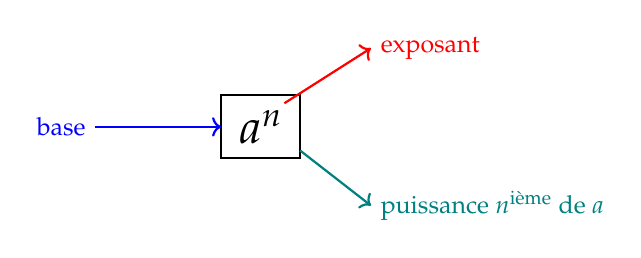
\begin{tikzpicture}[every node/.style={font=\small}]
    % Draw a box around a^n
    \node at (1.1,0) {\LARGE $a^n$};
    \draw[thick] (0.6,-0.4) rectangle (1.6,0.4);
    
    % Arrow to the left: base
    \draw[->, thick, blue] (-1,0) -- (0.6,0);
    \node[anchor=east, blue] at (-1,0) {base};
    
    % Arrow pointing to the exponent: exposant
    \draw[->, thick, red] (1.4,0.3) -- (2.5,1);
    \node[anchor=west, red] at (2.5,1) {exposant};
    
    % Arrow pointing to the whole expression: puissance n-ième
    \draw[->, thick, teal] (1.6,-0.3) -- (2.5,-1);
    \node[anchor=west, teal] at (2.5,-1) {puissance $n^{\text{ième}}$ de $a$};
\end{tikzpicture}
\end{center}
L'écriture $a^n$ se lit : $a$ à la puissnace $n$ \\
$a$ s'appelle la base, et $n$ s'appelle l'exposant
\end{Définition}

\begin{Exemple}
    \begin{multicols}{2}
        \begin{enumerate}
            \item $4^3 = 4\times4\times4 = 16\times 4 = 64$
            \item $2024^0 = 1$
            \item $105^1 = 105$
            \item $(-2)^{-3} = \displaystyle\frac{1}{(-2)^3} = -\displaystyle\frac{1}{8}$
            \item $(\sqrt{2})^3 = \sqrt{2}\times\sqrt{2}\times\sqrt{2} = 2\sqrt{2}$
        \end{enumerate}
    \end{multicols}
\end{Exemple}

\mysubsection{2}{Puissance de 10}
\begin{Proposition}
    Pour tout entier naturel $n$, on a :
    \begin{center}
         $10^n =\underset{\underbrace{\hspace{1.5cm}}_{n \text{ zéros }}}{1000000000}$ \hspace{1.5cm} et \hspace{1.5cm} $10^{-n} =\underset{\underbrace{\hspace{1.5cm}}_{n \text{ zéros }}}{0.0000000001}$
    \end{center}
\end{Proposition}

\begin{Proposition}
    Soit $ a $ et $ b $ deux nombres réels non nuls et soit $ n $ et $ p $ deux entiers relatifs :
    \begin{multicols}{3}
        \begin{itemize}
            \item $ a^n \times a^p = a^{n+p} $
            \item $ (a^n)^p = a^{np} $
            \item $ \displaystyle\frac{1}{a^p} = a^{-p} $
            \item $ a^n \times b^n = (a \times b)^n $
            \item $ \displaystyle\frac{a^n}{a^p} = a^{n-p} $
            \item $ \displaystyle\frac{a^n}{b^n} = \displaystyle\left(\frac{a}{b}\right)^n $
        \end{itemize}
    \end{multicols}
\end{Proposition}

\begin{Exemple}
    \begin{multicols}{2}
        \begin{enumerate}
            \item $5^{-2}\times5^4 = 5^{-2+4} = 5^2$
            \item $\displaystyle\frac{3^4}{3^5} = 3^{4-5} = 3^{-1} = \displaystyle\frac{1}{3}$
            \item $(2^3)^2 = 8^2 = 64$
            \item $2^3\times 3^3 = (2\times 3)^3 = 6^3 = 216$
            \item $\displaystyle\frac{15^3}{5^3} = \displaystyle(\frac{15}{5})^3 = 3^3 = 27$
        \end{enumerate}
    \end{multicols}
\end{Exemple}

\mysection{Les identités remarquables}

\mysubsection{1}{Développer un produit}
\begin{Définition}{Définition}
    \begin{itemize}
        \item Développer un produit, c’est l’écrire sous la forme d’une somme (ou d’une différence).
    \end{itemize}
\end{Définition}

\begin{Proposition}
    Soient $a,\ b,\ c$ et $d$ sont des nombres rationnels :
    \begin{multicols}{2}
        \begin{itemize}
            \item $a(b+c) = ab+ac$
            \item $a(b-c) = ab-ac$
            \item $(a+b)(c+d) = ac+ad+bc+bd$
        \end{itemize}
    \end{multicols}
\end{Proposition}

\begin{Exemple}
  \begin{multicols}{2}
       $\begin{array}{ll}
        A = & 6(x-4) \\
        A = & 6\times x - 6\times4 \\
        A = & 6x-24
    \end{array}$
    \vfill
    \columnbreak
     $\begin{array}{ll}
        B = & (x+2)(x-3) \\
        B = & x^2 -x\times3 + 2\times x - 2\times 3 \\
        B = & x^2 -3x + 2x - 6 \\
        B = & x^2 -x - 6 \\
    \end{array}$
  \end{multicols}
\end{Exemple}

\mysubsection{2}{Factorisation}
\begin{Définition}{Définition}
    Factoriser une somme (ou une différence), c’est l’écrire sous la forme d’un produit
\end{Définition}

\begin{Proposition}
    Soient $a,\ b$ et $k$ sont des nombres rationnels :
    \begin{multicols}{2}
        \begin{itemize}
            \item $ka+kb = k(a+b)$
            \item $ka-kb = k(a-b)$
        \end{itemize}
    \end{multicols}
\end{Proposition}

\begin{Exemple}
     \begin{multicols}{2}
       $\begin{array}{ll}
        A = & 4x^2 - 2x \\
        A = & 2x\times 2x - 2x\\
        A = & 2x(2x-1)
    \end{array}$
    \vfill
    \columnbreak
     $\begin{array}{ll}
        B = & (x + 1)(x + 2) - (2x - 3)(x + 2) \\
        B = & (x + 2)[(x + 1) - (2x - 3)] \\
        B = & (x + 2)(x + 1 - 2x + 3) \\
        B = & (x + 2)(-x + 4) \\
    \end{array}$
  \end{multicols}
\end{Exemple}

\mysubsection{3}{Identités remarquables}
\begin{Proposition}
    Soient $a$ et $b$ sont deux nombres rationnels : 
    \begin{itemize}
        \item $(a+b)^2 = a^2+2ab+b^2$
        \item $(a-b)^2 = a^2-2ab+b^2$
        \item $(a-b)(a+b) = a^2-b^2$
    \end{itemize}
\end{Proposition}

\begin{Exemple}
     \begin{multicols}{2}
       $\begin{array}{ll}
        A = & (x+3)^2  \\
        A = & x^2 + 2\times3\times x + 3^2\\
        A = & x^2 + 6x + 3^2\\
    \end{array}$
    \vfill 
    $\begin{array}{ll}
        C = & (2x+3)(2x-3)  \\
        C = & (2x)^2 - 3^2\\
        C = & 4x^2 - 9\\
    \end{array}$
    % \columnbreak
    
    $\begin{array}{ll}
        B = & (x-3)^2  \\
        B = & x^2 - 2\times3\times x + 3^2\\
        B = & x^2 - 6x + 3^2\\
    \end{array}$
  \end{multicols}
\end{Exemple}


\end{document}